\def\micro{\mu m}
\def\um{$\micro$ }
\def\degreesC{$\degree C$ }
\def\percent{$\%$ }
\documentclass[10pt,a4paper,oneside]{article}
\usepackage[left=2cm,right=2cm,top=2cm,bottom=2cm]{geometry}

\usepackage[dvipsnames]{xcolor}

%%  -------------------------------------------------------------------
%%      GDS II layer, regarding MOSIS SCMOS layer map
%%  -------------------------------------------------------------------
% GDS II #41 - P_WELL
\definecolor{pwell}{rgb}{1.0, 0.74, 0.53}   % macaroni and cheese
% GDS II #42 - N_WELL
\definecolor{nwell}{rgb}{0.61, 0.87, 1.0}  % columbia blue
\definecolor{pbase}{rgb}{1.0, 0.51, 0.26}  % mango tango
\definecolor{nbase}{rgb}{0.0, 0.75, 1.0}   % capri 
% GDS II #43 - ACITVE
\definecolor{active}{rgb}{0.9, 0.4, 0.38}   % light carmine pink
% GDS II #45 - N_PLUS_SELECT
\definecolor{nimplant}{rgb}{0.45, 0.76, 0.983}% maya blue
% GDS II #44 - P_PLUS_SELECT
\definecolor{pimplant}{rgb}{1.0, 0.51, 0.26}% mango tango
% GDS II #46 - POLY
\definecolor{poly}{rgb}{0.56, 0.93, 0.56}   % light green
% GDS II #25 - CONTACT
\definecolor{contact}{rgb}{0.83, 0.83, 0.83}% light gray
% GDS II #49 - METAL1
\definecolor{metal1}{rgb}{0.38, 0.31, 0.86} % majorelle blue
% GDS II #50 - VIA1
\definecolor{via1}{rgb}{0.83, 0.83, 0.83}   % light gray
% GDS II #51 - METAL2
\definecolor{metal2}{rgb}{0.04, 0.85, 0.32} % malachite
% GDS II #61 - VIA2
\definecolor{via2}{rgb}{0.83, 0.83, 0.83}   % light gray
% GDS II #63 - METAL3
\definecolor{metal3}{rgb}{0.98, 0.93, 0.37} % maize
% GDS II #30 - VIA3
\definecolor{via3}{rgb}{0.83, 0.83, 0.83}   % light gray
% GDS II #31 - METAL4
\definecolor{metal4}{rgb}{0.75, 0.25, 0.0}  % mahogany
% GDS II #32 - VIA4
\definecolor{via4}{rgb}{0.83, 0.83, 0.83}   % light gray
% GDS II #33 - METAL5
\definecolor{metal5}{rgb}{0.79, 0.08, 0.48} % magenta (dye)
% GDS II #36 - VIA5
\definecolor{via5}{rgb}{0.83, 0.83, 0.83}   % light gray
% GDS II #37 - METAL6
\definecolor{metal6}{rgb}{0.11, 0.35, 0.02} % lincoln green
% GDS II #29 - SILICIDE_BLOCK
\definecolor{silicide-block}{rgb}{0.98, 0.94, 0.9}  % linen
% GDS II #52 - GLASS
\definecolor{glass}{rgb}{1.0, 1.0, 0.88}    % light yellow
% GDS II #26 - PADS
\definecolor{pads}{rgb}{0.75, 1.0, 0.0}     % lime (color wheel)

\definecolor{resist}{rgb}{0.71, 0.4, 0.11}  % light brown

\definecolor{silicide}{rgb}{0.29, 0.33, 0.13}
\definecolor{titanium}{rgb}{0.8, 0.58, 0.46}

\def\OpacityLayout {0.5}

%
% physical
%
\definecolor{substrate}{rgb}{0.96, 0.94, 0.93}  % isabelline
\definecolor{nitride}{rgb}{1.0, 0.03, 0.0}
\definecolor{gateoxide}{rgb}{0.88, 1.0, 1.0}    % light cyan
\definecolor{isolationoxide}{rgb}{0.84, 0.79, 0.87}% languid lavender


\usepackage[utf8]{inputenc}
\usepackage[english]{babel}
\usepackage{forloop}
\usepackage{amsmath}
\usepackage{amsfonts}
\usepackage{amssymb}
\usepackage{gensymb}
\usepackage{mdframed}
\usepackage{graphicx}
\usepackage{tikz}
\usetikzlibrary{arrows,automata,shapes}
\usepackage[siunitx]{circuitikz}
\usepackage{makecell}
\usepackage{array}

\def\WaferClean{
\begin{tikzpicture}\node [fill=cyan, rounded corners=5pt] {Clean};\end{tikzpicture}}
\def\WaferSemiClean{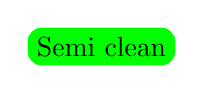
\begin{tikzpicture}\node [fill=green, rounded corners=5pt] {Semi clean};\end{tikzpicture}}
\def\WaferNonStandard{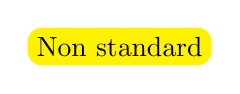
\begin{tikzpicture}\node [fill=yellow, rounded corners=5pt] {Non standard};\end{tikzpicture}}

\usepackage[colorlinks=true,linkcolor=blue,urlcolor=black,bookmarksopen=true]{hyperref}
\usepackage{bookmark}
\usepackage{hyperref}
\usepackage{sepfootnotes}
\usepackage{lipsum,tocloft} 
\usetikzlibrary{positioning}
\usetikzlibrary{patterns}

\usepackage[digital,srcmeas]{circdia}

\usepackage{float}
\floatstyle{boxed} 
\restylefloat{figure}

\title{CMOS in a nutshell}
\date{\today}
\author{	Hagen Sankowski}
\makeindex

\newcounter{ct}
\def\CrossSectionOnly{0.3}
\def\CrossAndTopSection{0.2}
\def\CrossAndTopSectionBig{0.3}
\def\VLSILayout{0.4}

\DeclareMathOperator\erfc{erfc}

\setlength{\parindent}{0pt} % get rid of annoying indents

\begin{document}
\begin{abstract}
	Copyright © 2017 LANCEVILLE TECHNOLOGY GROUP CO., LIMITED. All rights reserved. \\

This process is licensed under the Libre Silicon public license; you can redistribute it and/or modify it under the terms of the Libre Silicon public license
as published by the Libre Silicon alliance, either version 1 of the License, or (at your option) any later version.

This design is distributed in the hope that it will be useful, but WITHOUT ANY WARRANTY; without even the implied warranty of MERCHANTABILITY or FITNESS FOR A PARTICULAR PURPOSE.
See the Libre Silicon Public License for more details. \\

This document is part of the specification of the free silicon manufacturing standard for manufacturing the LibreSilicon standard logic cells\footnote{\url{https://github.com/chipforge/StdCellLib}} and related free technology nodes from the LibreSilicon project.

For this initial revision 0.1 a gate-first approach has been chosen which led to the choice of polysilicon as the gate electrode material because of the simplicity of the gate alignment.
For better isolation properties of the transistors and gates in overall a box-isolation approach has been chosen.
All of these choices have been made with the future scale down from the recent $1 \mu m$ to smaller structure sizes.
\textbf{This process is for manufacturing $1 \mu m$ only!}
But further releases which will have been tested with smaller structure sizes can be expected.

\end{abstract}
\newpage

\maketitle

This basic initial project is dedicated to the CMOS Technology only and for this reason two types of metal–oxide–semiconductor field-effect transistors (MOSFET) are required.

Historically, the first chips with MOSFETs on the mass market were p-channel MOSFETs in enhancement-mode.

\begin{figure}[H]
	\centering
	\begin{circuitdiagram}{20}{20}
		\power{15}{18.5}{U}{}  % power above pmos
		\wire{15}{18}{15}{16}   % wire above pmos
		\trans{penh}{13}{14}{R}{}{} % pmos -> right
		\Voltarrow{14}{18}{10}{16}{u}{$-V_{GS}$}
		\wire{15}{12}{15}{8}   % wire below pmos
		\resis{15}{5}{V}{$R_D$}{}  % resistor on drain
		\wire{15}{1}{15}{2}   % wire below pmos
		\ground{15}{0.5}{D}  % ground below resistor
		\othersrc[\sigsym{-rec}]{o}{5.5}{15.5}{H}{}{signal}
		\pin{9.5}{15.5}{R}{}	% pin in
		\ground{2.5}{0.5}{D}  % ground below signal source
		\wire{2.5}{1}{2.5}{15.5}   % wire below signal
		\junct{15}{10}   % dot
		\wire{15}{10}{16}{10}   % wire before out
		\pin{17}{10}{R}{out}	% pin out
	\end{circuitdiagram}
	\caption{enhancement-mode PMOS transistor use-case}
\end{figure}

The sectional view of a PMOS transistor in silicon is shown below
\begin{figure}[H]
	\centering
	\begin{tikzpicture}[node distance = 3cm, auto, thick,scale=0.5, every node/.style={transform shape}]
		% substrate
\fill[substrate] (0,0) rectangle (10,2);
\node at (2,0.5) {Si (p-type)};

% n-well
\fill[nwell] (1,0.75) rectangle (8.5,2);
\node at (5.75,1) {N-Well};

% body
\fill[nimplant] (1.5,1) rectangle (3,2);
\node at (2,1.5) {n+};
% source
\fill[pimplant] (3.5,1) rectangle (5,2);
\node at (4,1.5) {p+};
% drain
\fill[pimplant] (6.5,1) rectangle (8,2);
\node at (7,1.5) {p+};
%% gate:
% gate oxide
\fill[gateoxide] (4.8,2) rectangle (6.7,2.1);
% gate poly
\fill[gatemetal] (4.8,2.1) rectangle (6.7,2.2);

% metals ground
\fill[metal1] (2,2) rectangle (2.5,3);
\fill[metal1] (4,2) rectangle (4.5,3);
\fill[metal1] (0,3) rectangle (4.5,3.2); % connection pad GND

\fill[metal1] (5.5,2.2) rectangle (6,3);
\fill[metal1] (5.3,3) rectangle (6.2,3.2); % connection pad VG

\fill[metal1] (7,2) rectangle (7.5,3);
\fill[metal1] (6.8,3) rectangle (7.7,3.2); % connection pad VDD

% isolation oxides:
\fill[isolationoxide] (0,2) rectangle (2,3);
\fill[isolationoxide] (2.5,2) rectangle (4,3);
\fill[isolationoxide] (4.5,2) rectangle (4.8,3);
\fill[isolationoxide] (4.8,2.2) rectangle (5.5,3);
\fill[isolationoxide] (6,2.2) rectangle (6.7,3);
\fill[isolationoxide] (6.7,2) rectangle (7,3);
\fill[isolationoxide] (7.5,2) rectangle (10,3);

\node at (1.5,3.5) {Source};
\node at (5.5,3.4) {Gate};
\node at (7.5,3.4) {Drain};

% trench
\fill[isolationoxide] (0,0.75) rectangle (1,2);
\fill[isolationoxide] (8.5,0.75) rectangle (10,2);;
	\end{tikzpicture}
	\caption{Sectional view of a PMOS transistor}
\end{figure}

Historically later, faster chips with MOSFETs on the mass market were marked as n-channel MOSFETs in enhancement mode also.

\begin{figure}[H]
	\centering
	\begin{circuitdiagram}{20}{20}
		\power{15}{18.5}{U}{}  % power above resistor
		\wire{15}{17}{15}{18}   % wire above resistor
		\resis{15}{14}{V}{$R_D$}{}  % resistor on drain
		\wire{15}{11}{15}{8}   % wire between resistor and nmos
		\trans{nenh}{13}{6}{R}{}{} % nmos -> right
		\Voltarrow{10}{4}{14}{1}{d}{$+V_{GS}$}
		\wire{15}{1}{15}{4}   % wire below nmos
		\ground{15}{0.5}{D}  % ground below nmos
		\othersrc[\sigsym{rec}]{o}{5.5}{4.5}{H}{}{signal}
		\pin{9.5}{4.5}{R}{}	% pin in
		\ground{2.5}{0.5}{D}  % ground below signal source
		\wire{2.5}{1}{2.5}{4.5}   % wire below signal
		\junct{15}{10}   % dot
		\wire{15}{10}{16}{10}   % wire before out
		\pin{17}{10}{R}{out}	% pin out
	\end{circuitdiagram}
	\caption{enhancement-mode NMOS transistor use-case}
\end{figure}

The sectional view of a NMOS transistor in silicon is shown here also.
\begin{figure}[H]
	\centering
	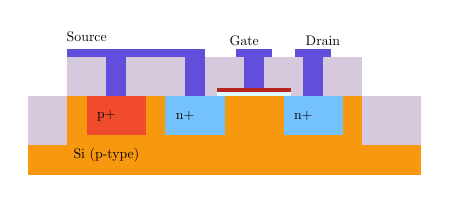
\begin{tikzpicture}[node distance = 3cm, auto, thick,scale=0.5, every node/.style={transform shape}]
		% substrate
\fill[YellowOrange] (0,0) rectangle (10,2);
\node at (2,0.5) {Si (p-type)};
% body
\fill[RedOrange] (1.5,1) rectangle (3,2);
\node at (2,1.5) {p+};
% source
\fill[nimplant] (3.5,1) rectangle (5,2);
\node at (4,1.5) {n+};
% drain
\fill[nimplant] (6.5,1) rectangle (8,2);
\node at (7,1.5) {n+};
%% gate:
% gate oxide
\fill[gateoxide] (4.8,2) rectangle (6.7,2.1);
% gate poly
\fill[BrickRed] (4.8,2.1) rectangle (6.7,2.2);
% metals ground
\fill[metal1] (2,2) rectangle (2.5,3);
\fill[metal1] (4,2) rectangle (4.5,3);
\fill[metal1] (1,3) rectangle (4.5,3.2); % connection pad GND

\fill[metal1] (5.5,2.2) rectangle (6,3);
\fill[metal1] (5.3,3) rectangle (6.2,3.2); % connection pad VG

\fill[metal1] (7,2) rectangle (7.5,3);
\fill[metal1] (6.8,3) rectangle (7.7,3.2); % connection pad VDD

% isolation oxides:
\fill[isolationoxide] (1,2) rectangle (2,3);
\fill[isolationoxide] (2.5,2) rectangle (4,3);
\fill[isolationoxide] (4.5,2) rectangle (4.8,3);
\fill[isolationoxide] (4.8,2.2) rectangle (5.5,3);
\fill[isolationoxide] (6,2.2) rectangle (6.7,3);
\fill[isolationoxide] (6.7,2) rectangle (7,3);
\fill[isolationoxide] (7.5,2) rectangle (8.5,3);

%field oxides:
% trench
\fill[isolationoxide] (0,0.75) rectangle (1,2);
\fill[isolationoxide] (8.5,0.75) rectangle (10,2);

\node at (1.5,3.5) {Source};
\node at (5.5,3.4) {Gate};
\node at (7.5,3.4) {Drain};
	\end{tikzpicture}
	\caption{Sectional view of a NMOS transistor}
\end{figure}

Both technologies, the older PMOS as the newer NMOS, have the same disadvantage. Every time, the transistor is switched on, the current between drain and source of the transistor is limited by the resistor on drain only. Higher currents here means higher power consumption for the chip where the transistors are integrated as well. If the transistors are switched off, no current flows between drain and source anymore, the power consumption of the chip also goes low.
Et viol\'{a}, the US-Patent with Number 3356858\footnote{\url{https://www.google.com/patents/US3356858}} changed the world and combines both technologies to the new complementary metal-oxide-semiconductor (CMOS) technology. Instead of every transistor working against a weak resistor, the transistor works against a complementary switched-off transistor. With the eyes of our antecessor CMOS doubles the transistor count, but contemporary chips all are built in CMOS.

\begin{figure}[H]
	\centering
	\begin{circuitdiagram}{20}{20}
		\power{15}{18.5}{U}{}  % power above pmos 
		\wire{15}{16}{15}{18}   % wire above pmos
		\trans{penh}{13}{14}{R}{}{} % pmos -> right
		\Voltarrow{14}{18}{10}{16}{u}{$-V_{GS}$}
		\wire{15}{8}{15}{12}   % wire between pmos and nmos
		\trans{nenh}{13}{6}{R}{}{} % nmos -> right
		\Voltarrow{10}{4}{14}{1}{d}{$+V_{GS}$}
		\wire{15}{1}{15}{4}   % wire below nmos
		\ground{15}{0.5}{D}  % ground below nmos
		\othersrc[\sigsym{rec}]{o}{5}{10}{H}{}{signal}
		\pin{9}{10}{R}{}	% pin in
		\wire{9.5}{10}{10}{10}   % wire before gates
		\wire{10}{15.5}{10}{4.5}   % wire between gates
		\junct{10}{10}   % dot
		\ground{2}{0.5}{D}  % ground below signal source
		\wire{2}{1}{2}{10}   % wire below signal
		\junct{15}{10}   % dot
		\wire{15}{10}{16}{10}   % wire before out
		\pin{17}{10}{R}{out}	% pin out
	\end{circuitdiagram}
	\caption{complementary PMOS and NMOS transistor couple use-case}
\end{figure}

Below the sectional view of the inverter circuitry can be seen.
For the run through of this process we will use this cross section diagram as reference.
\begin{figure}[H]
	\centering
	\begin{tikzpicture}[node distance = 3cm, auto, thick,scale=0.5, every node/.style={transform shape}]
		% substrate
\fill[YellowOrange] (0,0) rectangle (20,2);
\node at (2,0.5) {Si (p-type)};
% n-well
\fill[nwell] (1,0.75) rectangle (8.5,2);
\node at (5.75,1) {N-Well};
% body
\fill[nimplant] (1.5,1) rectangle (3,2);
\node at (2,1.5) {n+};
% source
\fill[RedOrange] (3.5,1) rectangle (5,2);
\node at (4,1.5) {p+};
% drain
\fill[RedOrange] (6.5,1) rectangle (8,2);
\node at (7,1.5) {p+};
%% gate:
% gate oxide
\fill[gateoxide] (4.8,2) rectangle (6.7,2.1);
% gate poly
\fill[BrickRed] (4.8,2.1) rectangle (6.7,2.2);
% isolation oxides:
\fill[isolationoxide] (1,2) rectangle (2,3);
\fill[isolationoxide] (2.5,2) rectangle (4,3);
\fill[isolationoxide] (4.5,2) rectangle (4.8,3);
\fill[isolationoxide] (4.8,2.2) rectangle (5.5,3);
\fill[isolationoxide] (6,2.2) rectangle (6.7,3);
\fill[isolationoxide] (6.7,2) rectangle (7,3);
\fill[isolationoxide] (7.5,2) rectangle (8.5,3);

%trenches
\fill[isolationoxide] (0,0.75) rectangle (1,2);
\fill[isolationoxide] (8.5,0.75) rectangle (11.5,2);
\fill[isolationoxide] (19,0.75) rectangle (20,2);

%%% nmos:
% body
\fill[RedOrange] (17,1) rectangle (18.5,2);
\node at (18,1.5) {p+};
% source
\fill[nimplant] (15,1) rectangle (16.5,2);
\node at (16,1.5) {n+};
% drain
\fill[nimplant] (12,1) rectangle (13.5,2);
\node at (13,1.5) {n+};

%% gate:
% gate oxide
\fill[gateoxide] (13.3,2) rectangle (15.2,2.1);
% gate poly
\fill[BrickRed] (13.3,2.1) rectangle (15.2,2.2);

% metals
\fill[gatemetal] (17.5,2) rectangle (18,3);
\fill[gatemetal] (15.5,2) rectangle (16,3);
\fill[gatemetal] (15.5,3) rectangle (19,3.2); % connection pad GND

\fill[gatemetal] (14,2.2) rectangle (14.5,3);
\fill[gatemetal] (13.8,3) rectangle (14.7,3.2); % connection pad VG

\fill[gatemetal] (12.5,2) rectangle (13,3);
\fill[gatemetal] (12.3,3) rectangle (13.2,3.2); % connection pad VDD

\fill[gatemetal] (2,2) rectangle (2.5,3);
\fill[gatemetal] (4,2) rectangle (4.5,3);
\fill[gatemetal] (1,3) rectangle (4.5,3.2); % connection pad GND

\fill[gatemetal] (5.5,2.2) rectangle (6,3);
\fill[gatemetal] (5.3,3) rectangle (6.2,3.2); % connection pad VG

\fill[gatemetal] (7,2) rectangle (7.5,3);
\fill[gatemetal] (6.8,3) rectangle (7.7,3.2); % connection pad VDD

% isolation oxides:
\fill[isolationoxide] (18,2) rectangle (19,3);
\fill[isolationoxide] (16,2) rectangle (17.5,3);
\fill[isolationoxide] (15.2,2) rectangle (15.5,3);
\fill[isolationoxide] (14.5,2.2) rectangle (15.2,3);
\fill[isolationoxide] (13.3,2.2) rectangle (14,3);
\fill[isolationoxide] (13,2) rectangle (13.3,3);
\fill[isolationoxide] (11.5,2) rectangle (12.5,3);

\node at (1.5,3.5) {VDD};
\node at (16.5,3.5) {Ground};
\node at (5.5,3.4) {Input};
\node at (14,3.4) {Input};
\node at (7,3.4) {Output};
\node at (12.5,3.4) {Output};

\node at (0.5,1.5) {Trench};
\node at (9.5,1.5) {Trench};
\node at (19.5,1.5) {Trench};
	\end{tikzpicture}
	\caption{Sectional view of a NMOS-PMOS transistor circuit}
\end{figure}

\end{document}

